\begin{figure}[H]
\centering
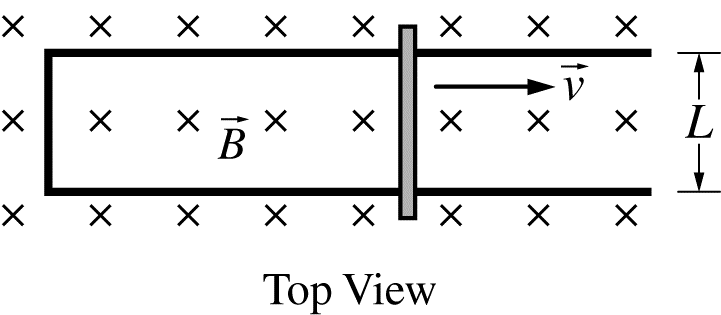
\includegraphics[scale=0.3]{images/img-006-009.png}
\end{figure}

% Multiple Choice Question 9
\begin{questions}\setcounter{question}{8}\question
A copper rod of resistance $R$ is in electrical contact with a frictionless U-shaped rail of width $L$ and negligible resistance. The rod is pulled to the right at a constant velocity $\vec{v}$. A magnetic field $\vec{B}$ is directed into the page, as shown in the figure above. Under these conditions, the electric power dissipated in the rod is $P$. If the velocity of the rod is doubled and the magnetic field strength is reduced by half, the power dissipated in the rod is

\begin{oneparchoices}
\choice $P / 4$
\choice $P / 2$
\choice $P$
\choice $2P$
\choice $4P$
\end{oneparchoices}\end{questions}

